\documentclass[10pt,letterpaper]{article}
\usepackage[margin=.75in]{geometry}
\usepackage{amsmath,amssymb,graphicx,booktabs,xcolor,hyperref,fancyhdr}
\definecolor{navy}{HTML}{17364B}
\hypersetup{colorlinks=true,urlcolor=navy}
\pagestyle{fancy}\fancyhf{}\lhead{\small WEIGHTED DECAY EXPERIMENTS}\rhead{\small Numerical refinement}\cfoot{\thepage}
\setlength{\headheight}{14pt}\setlength{\parindent}{0pt}\setlength{\parskip}{5pt}
\newcommand{\RefinedRows}{Homogeneous & Gaussian & 0.00731 & 1.11\% & 0.18\% \\
Homogeneous & Compact bump & 0.00677 & 0.43\% & 0.03\% \\
Homogeneous & Near degeneracy & 0.00499 & 1.62\% & 0.24\% \\
Homogeneous & Random (33) & 0.00618 & 1.61\% & 0.29\% \\
Inhomogeneous & Gaussian & 0.00468 & 0.01\% & 0.05\% \\
Inhomogeneous & Compact bump & 0.00431 & 0.00\% & 0.54\% \\
Inhomogeneous & Near degeneracy & 0.00344 & 1.36\% & 0.01\% \\
Inhomogeneous & Random (33) & 0.00415 & 0.00\% & 0.04\% \\}
\newcommand{\ObservedResult}{The inhomogeneous Gaussian and random packet ratios begin to flatten: from $t=8$ to $16$ they grow by 3.42\% and 0.78\%, respectively. The near-degeneracy ratios continue to rise more visibly, as do several homogeneous cases. This suggests different transient time scales; it does not establish their eventual behavior.}
\newcommand{\CheckResult}{Across all 24 checked case--time combinations, the largest peak changes are 1.62\% under domain enlargement and 0.94\% under grid refinement. All pass the exploratory 2\% screen.}

\begin{document}
{\color{navy}\LARGE Testing the decay inequality}\par
{\large Clearer plots and a longer, larger-domain experiment}\par
\smallskip
\textbf{Research question.} Does the weighted solution obey the paper's proposed
power-law bound across different initial fields? The earlier optical-envelope
plots showed spreading. This experiment measures the quantity in the inequality.

We work directly in the canonical coordinates of (6.2), using
\[
 S(t)f=\mathcal F^{-1}(e^{itw}\widehat f),\qquad
 w=k_x^3+3s k_x(k_y^2+k_z^2)+3\beta(k_y^2+k_z^2).
\]
The two cases are $(s,\beta)=(-1,0)$ and $(+1,1)$, matching the minus homogeneous
and plus inhomogeneous symbols used in the proofs of Propositions 6.2--6.3.
We follow those proofs' positive phase convention; equation (6.1) prints inconsistent
signs. No transformation from the original optical coordinates is needed here.

For $\alpha=1/2$ and $p=\infty$, the diagnostic is
\[
 R(t;f)=\frac{t^{7/6}\big\||D_x+\beta|^{1/2}S(t)f\big\|_\infty}{\|f\|_1}.
\]
The inequality asserts $R(t;f)\le C$ with $C$ independent of $t$ and $f$ at fixed
parameters. The multiplier is $|k_x+\beta|^{1/2}$, not an ordinary spatial derivative.
Inputs are normalized to discrete $L^1=1$ on each grid.

\textbf{How to read the plots.} A flat ratio corresponds to weighted decay like
$t^{-7/6}$ over that interval. A falling ratio indicates faster decay there; a rising
ratio indicates slower decay there. \textbf{A rising but bounded ratio is compatible
with the theorem.} No horizontal ``failure threshold'' is drawn because the theorem's
constant is unspecified. Finite curves cannot establish unbounded growth.

\begin{center}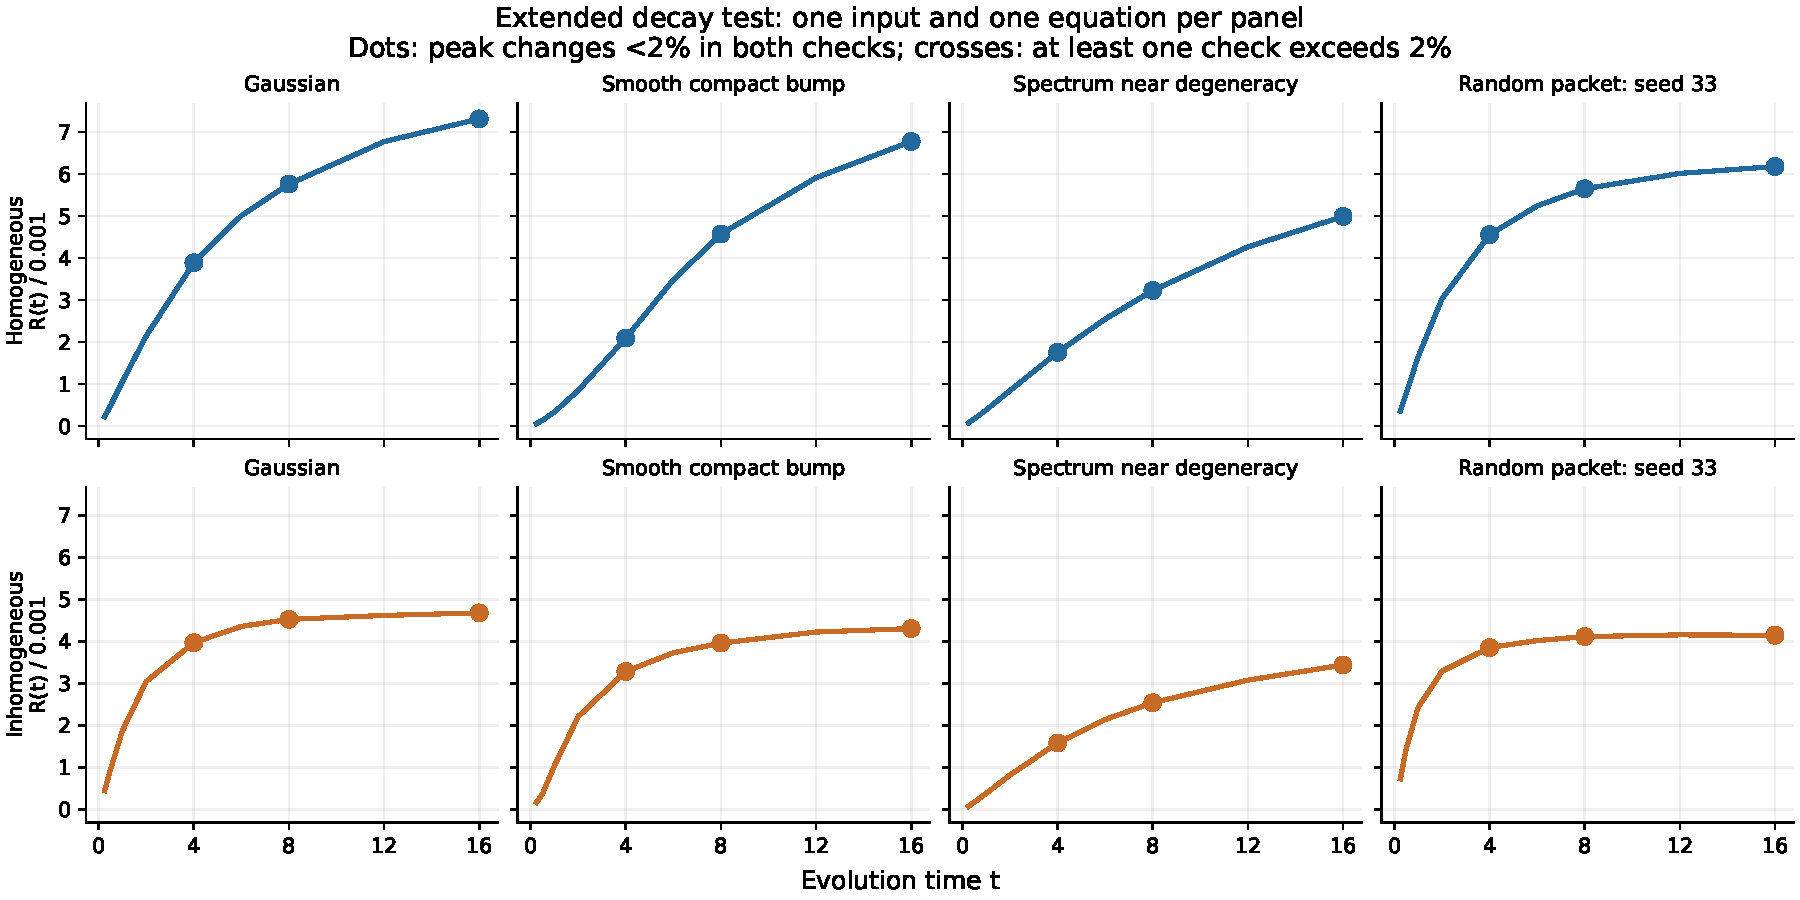
\includegraphics[width=\linewidth]{../results/decay_dataset/refined_clear.pdf}\end{center}
\textbf{Figure 1.} Each panel contains one family and one equation. Curves use a
length-288 periodic cube at spacing 1; vertical values are shown in units of $0.001$.
At $t=4,8,16$, dots indicate less than 2\% peak change in both tested refinements;
crosses indicate at least one larger change. Intermediate times are not independently
checked. The 2\% rule is a screening criterion, not a rigorous error bound.

\newpage
\section*{The broader collection of artificial inputs}
\begin{center}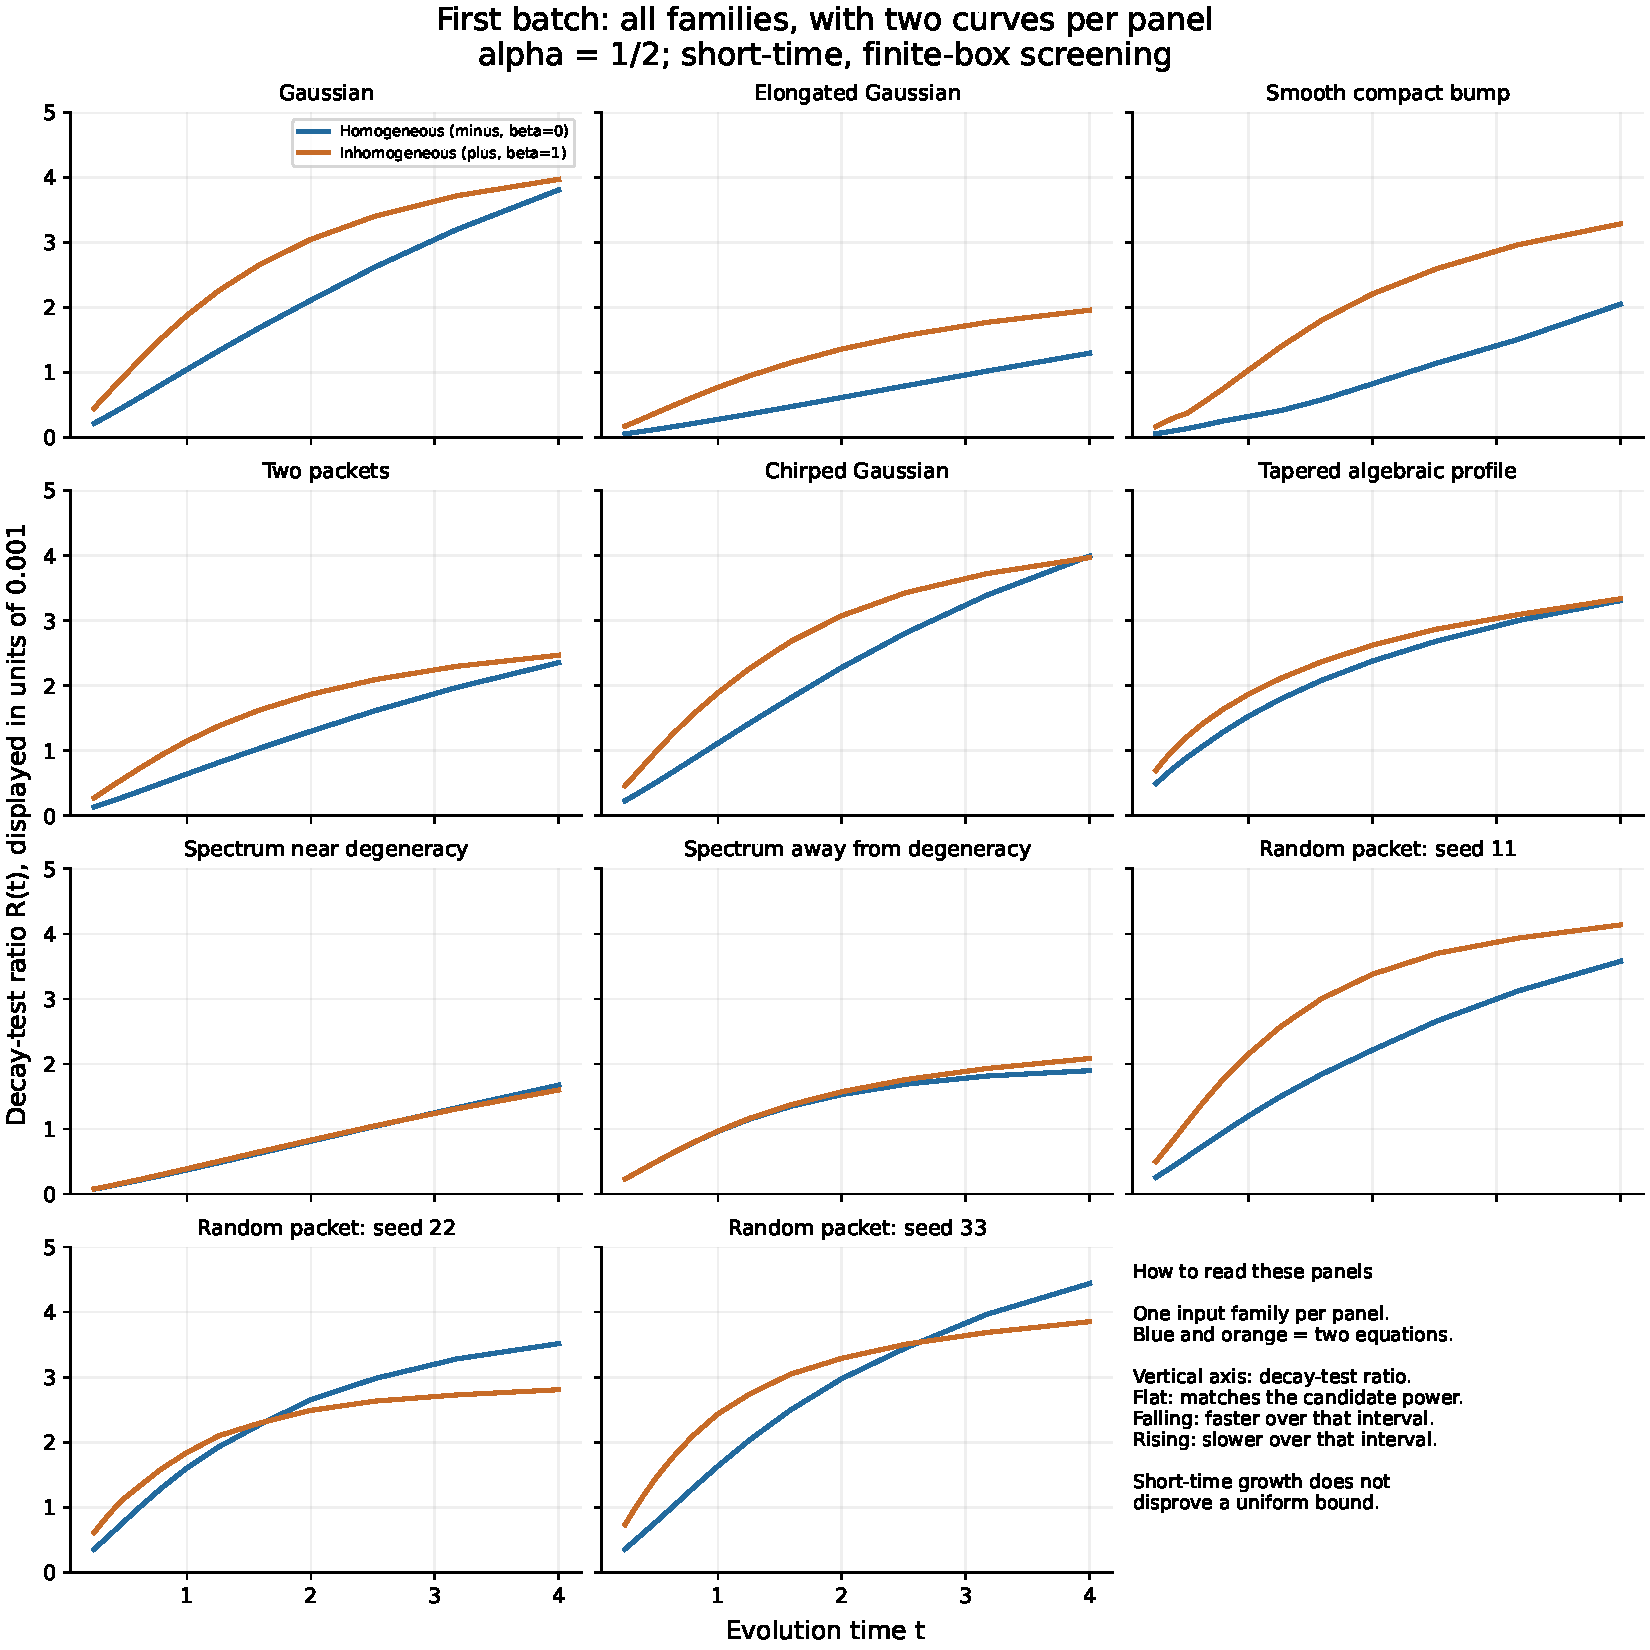
\includegraphics[width=.95\linewidth]{../results/decay_dataset/families_clear.pdf}\end{center}
\textbf{Figure 2.} Eleven input families, with two equation variants per panel.
These are the original short-time results on a length-96 box, replotted without
eleven overlapping curves. Their domain sensitivity remains as recorded in the
first batch; the new layout does not make them converged whole-space results.

All recipes define continuous functions that can be resampled on a different grid.
The collection includes Gaussian and anisotropic packets, a smooth compact bump,
two packets, a chirped phase, a tapered algebraic profile, spectral centers near and
away from $k_x=-\beta$, and three seeded random packets. Near/away-degeneracy inputs
depend on $\beta$ and therefore differ between the two equation variants. Random
fields combine twelve modes with fixed seeds and a Gaussian spatial window.

\newpage
\section*{What was refined, and what the results support}
We extend four families in both regimes to $t=16$, four times the first batch's
maximum time. Gaussian is the reference, the compact bump has a broader spectrum,
the near-degeneracy packet targets the multiplier's cusp, and seed 33 represents
the random collection. This is a targeted follow-up, not an exhaustive data search.

Domain checks compare lengths 96, 192, and 288 at spacing 1. A separate length-192
grid with spacing $2/3$ checks resolution. Every comparison uses the same continuum
recipe, normalized using its own grid quadrature. The table gives results at $t=16$;
machine-readable files also include $t=4,8$ and complex-field errors on a common cube.

\begin{center}\small
\begin{tabular}{llrrr}\toprule
Equation & Input & $R(16)$ & Domain peak change & Grid peak change\\\midrule
\RefinedRows
\bottomrule\end{tabular}
\end{center}
Domain peak change compares lengths 192 and 288; grid peak change compares
spacings 1 and $2/3$ at length 192. Peak comparisons use each grid's full sampled
maximum, not a fixed spatial point. The plotted length-288 field is not itself
also refined to spacing $2/3$, so the checks do not establish joint convergence.

\textbf{Observed behavior.} \ObservedResult

\textbf{Numerical qualification.} \CheckResult
The fractional multiplier can produce long spatial tails, and errors can vary
nonmonotonically with box size near its cusp. A field's relative $L^2$ difference
and its maximum-amplitude difference are distinct: this follow-up prioritizes the
maximum because it appears in the inequality, while retaining both diagnostics.

\textbf{Inference.} These experiments do not establish a faster universal decay
rate, a theorem constant, or a counterexample. A convincing candidate violation
would require a controlled sequence of times or normalized inputs with increasing
ratios that survives numerical refinement. A short transient slope is insufficient.
Cases that fail the peak checks should be refined before being interpreted as
evidence about the whole-space bound.

\textbf{Data and reproducibility.} Run \texttt{python3 decay\_dataset.py}, then
\texttt{python3 refine\_decay.py}. Results are in
\texttt{results/decay\_dataset/}: \texttt{refined\_decay.csv},
\texttt{refinement\_checks.json}, \texttt{REFINEMENT.md}, and the plotted figures.
The first batch's inputs remain available as complex-valued NPZ arrays.
These are artificial inputs. CDIP buoy observations have been identified as a
possible source, but are not imported or presented as three-dimensional measurements.

\textbf{Source.} R. Mosincat, D. Pilod, and J.-C. Saut,
\emph{On Third Order Nonlinear Schr\"odinger Equations}, supplied manuscript
\texttt{Dysthe3D-2.pdf}, Section 6. This supplement follows the stated estimates
as research targets, without claiming to resolve the manuscript's proof details.
\newpage
\newcommand{\LongRows}{Homogeneous & Gaussian & 0.00917 & 0.00999 & 1.043 \\
Homogeneous & Near degeneracy & 0.00833 & 0.00888 & 1.074 \\
Inhomogeneous & Gaussian & 0.00407 & 0.00372 & 1.293 \\
Inhomogeneous & Near degeneracy & 0.00558 & 0.00586 & 1.096 \\}
\newcommand{\LongDomain}{0.141\%}
\newcommand{\LongQuad}{0.020\%}
\newcommand{\LongEdge}{0.586\%}

\section*{Extension through $t=256$}
We now evaluate $t=16,32,64,128,256$ for the Gaussian and near-degeneracy packet,
in both canonical equation regimes, with $\alpha=1/2$. These two profiles admit
an efficient whole-space transverse integration. Other artificial families have
not yet been extended to $256$ by this method.

\begin{center}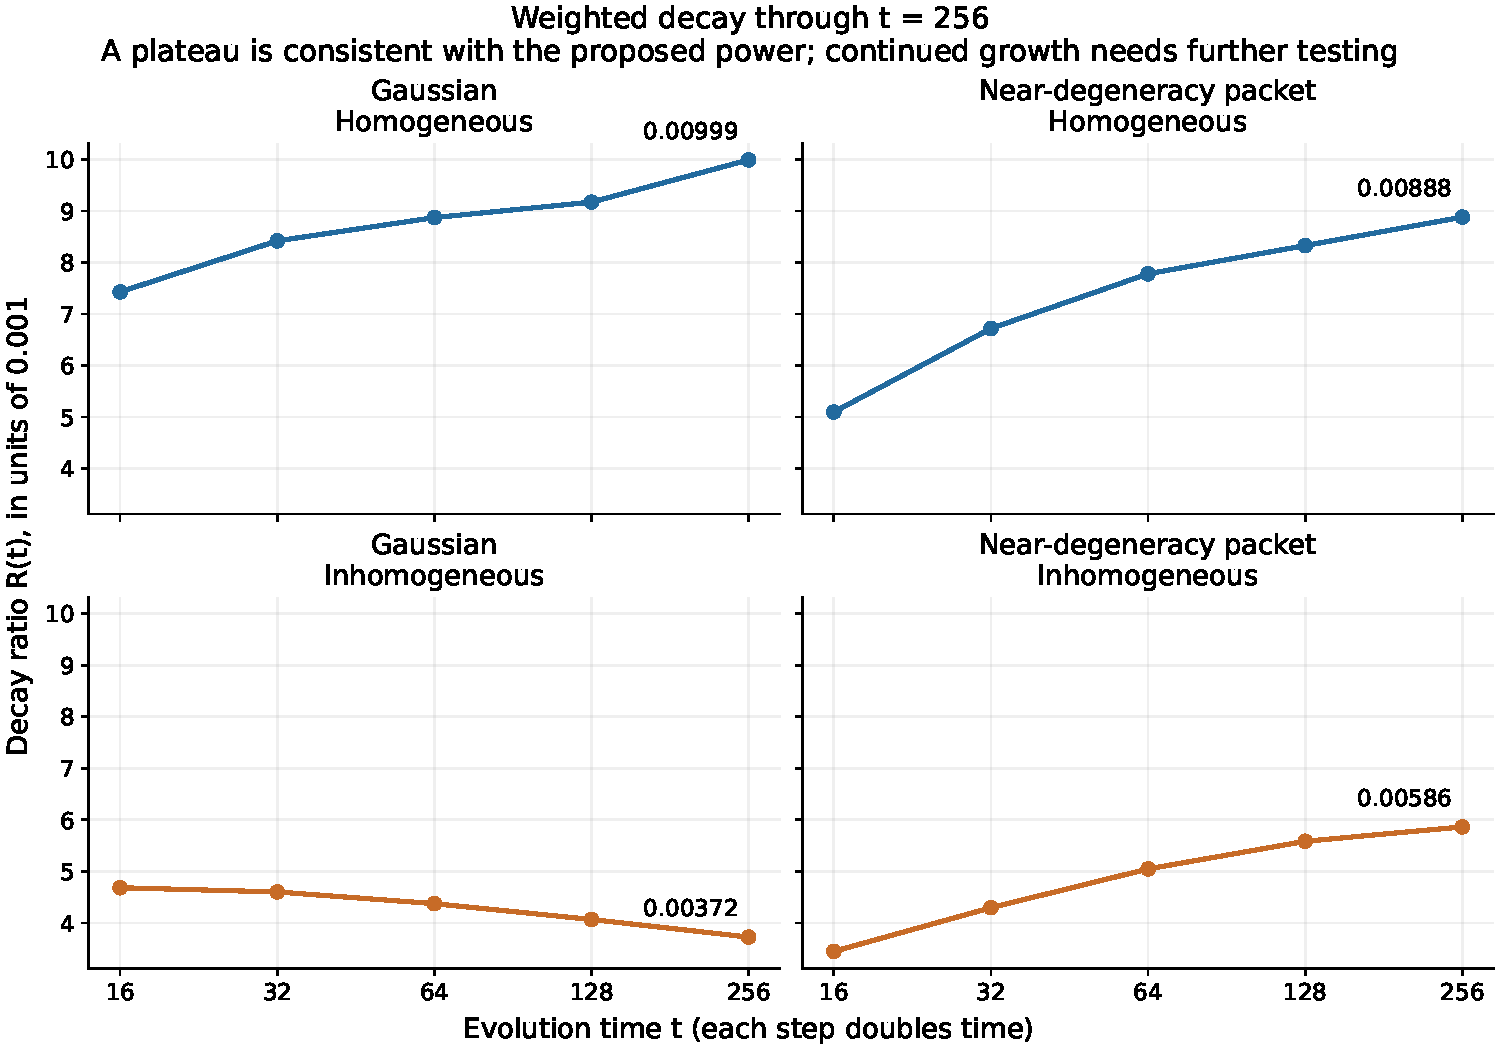
\includegraphics[width=\linewidth]{../results/long_time/decay_256.pdf}\end{center}
\textbf{Figure 3.} One curve per panel, with time doubling at each marker.
The ordinate is the same ratio $R(t)$ as before, displayed in units of $0.001$;
endpoint labels give its unscaled value. A downward curve means faster weighted
decay than $t^{-7/6}$ over that interval. An upward curve can still approach a
finite limit and does not by itself contradict the inequality.

\begin{center}\small
\begin{tabular}{llrrr}\toprule
Equation & Input & $R(128)$ & $R(256)$ & Effective exponent\\\midrule
\LongRows
\bottomrule\end{tabular}\end{center}
For weighted maximum $M(t)$, the last column is
$\gamma_{128,256}=-\log[M(256)/M(128)]/\log2$. It describes only the last time
doubling; it is not a fitted asymptotic exponent or a new uniform bound. The
paper's comparison exponent at $\alpha=1/2$ is $7/6\simeq1.167$.

\textbf{Finding.} The inhomogeneous Gaussian ratio decreases at late times.
The other three ratios increase over the last doubling, by different amounts.
None of these finite curves establishes a counterexample. The next question is
whether the rising ratios approach a finite limit or continue growing through
successive, independently checked time doublings.

\newpage
\section*{How the long-time calculation is checked}
Let $r=\sqrt{y^2+z^2}$ and use the exactly $L^1$-normalized initial profile
\[
 f(x,r)=\frac{\exp[-x^2/(2\sigma_x^2)-r^2/(2\sigma_y^2)]e^{iqx}}
 {(2\pi)^{3/2}\sigma_x\sigma_y^2}.
\]
The Gaussian has $(\sigma_x,\sigma_y,q)=(3,3,0)$; the near-degeneracy packet
has $(6,3,-\beta)$. Analytically integrating both transverse Fourier variables
reduces the weighted field to
\[
 W(x,r,t)=\frac1{4\pi^2}\int_{\mathbb R}
 \frac{|k+\beta|^{1/2}}{d(k,t)}
 \exp\!\left[-\frac{\sigma_x^2(k-q)^2}{2}+i(tk^3+kx)
             -\frac{r^2}{2d(k,t)}\right]dk,
 \qquad d(k,t)=\sigma_y^2-6it(sk+\beta).
\]
This is the same three-coordinate linear solution for these inputs. Only the
evaluation method changes. The transverse directions are treated on the whole
space; a longitudinal FFT quadrature evaluates many $x$ locations efficiently.
Radial symmetry reduces the spatial peak search to $(x,r)$.

\begin{center}\begin{tabular}{lrrrr}\toprule
Check & $x$ period & $\Delta x$ & Max. $r$ & $\Delta r$\\\midrule
Base & 4096 & 0.5 & 512 & 4\\
Expanded & 8192 & 0.5 & 1024 & 4\\
Refined & 8192 & 0.25 & 1024 & 2\\
Extra expansion at $t=256$ & 32768 & 0.25 & 2048 & 2\\\bottomrule
\end{tabular}\end{center}
The full $(x,r)$ search is followed by local optimization of the peak. At $256$,
the extra expansion changes the sampled peak by at most \LongDomain. An independent
adaptive quadrature of the integral above agrees with the complex field at each
final candidate peak to within \LongQuad\ relative error. The largest sampled
search-boundary amplitude is \LongEdge\ of its case's peak. These checks are
numerical evidence, not a certification that no larger unsampled peak exists.

\textbf{Why the previous box was inadequate.} At $t=256$, the inhomogeneous
near-degeneracy maximum lies around $x=-841$. It would be outside even the
length-288 box used for the earlier $t\le16$ runs. Extending time without changing
the spatial computation would therefore be unreliable.

\textbf{Remaining limits.} The Gaussian-specific reduction cannot be applied
unchanged to arbitrary measured fields or every artificial recipe. The adaptive
quadrature checks selected peak locations; the global search remains finite and
sampled. The two-dimensional radial search, local optimizer status, boundary ratios,
and domain/resolution comparisons are all recorded to make these limits reviewable.

\textbf{Reproduce.} Run \texttt{python3 long\_time\_decay.py}, followed by
\texttt{python3 report/make\_long\_time\_tables.py}. Results and the graph are under
\texttt{results/long\_time/}; compile \texttt{report/decay\_refinement.tex} for this
updated supplement. Source: the same manuscript, canonical symbols (6.2) and
weighted estimates in Propositions 6.2--6.3.

\newpage
\newcommand{\SpatialRows}{Homogeneous & Gaussian & 0.0130\% & 0.0000\% & 0.0046\% & 0.0025\% \\
Homogeneous & Near degeneracy & 0.0020\% & 0.0000\% & 0.0007\% & 0.0003\% \\
Inhomogeneous & Gaussian & 0.0001\% & 0.0000\% & 0.0000\% & 0.0000\% \\
Inhomogeneous & Near degeneracy & 0.0033\% & 0.0000\% & 0.0026\% & 0.0004\% \\}
\newcommand{\SpatialLocations}{Homogeneous & Gaussian & 0.0099887 & -20.7469 & 0.0000 & 0.00000 \\
Homogeneous & Near degeneracy & 0.0088803 & 7.7961 & 6.5381 & 0.00079 \\
Inhomogeneous & Gaussian & 0.0037238 & -8.9154 & 0.0000 & 0.00002 \\
Inhomogeneous & Near degeneracy & 0.0058621 & -841.2464 & 0.0000 & 0.00021 \\}
\newcommand{\SpatialLocationDrift}{0.00079}
\newcommand{\SpatialPeakDrift}{0.00459\%}
\newcommand{\SpatialQuadTighten}{$3.67\times10^{-12}\%$}
\newcommand{\SpatialBoundary}{0.00516\%}
\newcommand{\SpatialPassed}{4}

\section*{Stronger spatial reliability at $t=256$}
\textbf{Purpose.} Hold time, input, and $\alpha=1/2$ fixed, and vary the spatial
computation. This audit separates longitudinal enlargement from transverse
enlargement. It tests whether the four reported candidate maxima stabilize to
an exploratory relative tolerance of $0.1\%$.

The longitudinal period increases from 32,768 to 65,536 while the radial limit
stays at 2,048. We then search the additional annulus out to radius 4,096.
Finally, we double the longitudinal period again to 131,072, retaining the
larger radial limit. Every broad scan keeps $\Delta x=0.25$ and $\Delta r=2$.
The baseline is the saved final scan from the preceding experiment.

\begin{center}\small
\begin{tabular}{llrrrr}\toprule
Equation & Input & First $L$ change & Radius change & Second $L$ change & Integral check\\\midrule
\SpatialRows
\bottomrule\end{tabular}\end{center}
The three domain columns compare sampled peak magnitudes before and after the
stated expansion. The integral check compares the final Fourier-quadrature field
to an independently evaluated non-periodic integral at the refined candidate peak.
Percentages use the newer or independent result as the denominator. Values are rounded.

\textbf{Result.} \SpatialPassed\ of four cases pass the $0.1\%$ peak screen.
This includes the two longitudinal expansions, the transverse expansion, the
final locally optimized peak drift, and the independent integral check.
The largest change in locally optimized peak magnitude between the final two
periods is \SpatialPeakDrift.

\begin{center}\small
\begin{tabular}{llrrrr}\toprule
Equation & Input & Refined $R(256)$ & $x$ & $r$ & Location drift\\\midrule
\SpatialLocations
\bottomrule\end{tabular}\end{center}
Locations are continuous-coordinate candidate maxima from the independent
integral optimization. The drift is the Euclidean distance in $(x,r)$ between
local peak optimizations at the final two longitudinal periods. Its maximum is
\SpatialLocationDrift. Axial symmetry means a nonzero $r$ represents a ring of
equivalent points, not a unique three-dimensional location.

\textbf{Additional checks.} Local optimization starts from the broad search's
largest sample and refines both $x$ and $r$. Increasing the independent
integral's Gauss--Legendre order from 256 to 512 per panel changes the complex field by
at most \SpatialQuadTighten\ relative to the tighter result. Its integration
interval is split at the fractional multiplier cusp and into 64 Gaussian-frequency
panels. On each side, $k=-\beta\pm u^2$ removes the square-root cusp from the
integration variable. Fixed-order quadrature with an order-doubling check replaces
adaptive quadrature, which issued convergence warnings during local searches.
The largest sampled search-boundary amplitude is \SpatialBoundary\ of
the corresponding peak. Optimizer status and all intermediate measurements are
saved in the per-case JSON records.

\textbf{What we can now say.} At this time and for these four inputs, the peak
values have stronger numerical support from separate domain enlargements,
continuous local refinement, stable locations, and independent integration.
This improves confidence in the reported decay ratios. It does not prove the
maximum is global over all of $\mathbb R^3$, establish an asymptotic decay rate,
or extend reliability to other inputs, values of $\alpha$, or later times.

\textbf{Remaining spatial limitation.} The broad radial mesh is still spaced by
2; refinement is local to the identified maximum, not a global halving of every
cell. A missed narrow peak or a remote maximum is not excluded by these checks.
The report therefore claims numerical spatial stability of the identified peaks,
not a certified supremum.

\textbf{Reproduce.} Run \texttt{python3 spatial\_reliability.py}, then
\texttt{python3 report/make\_spatial\_tables.py}. Results, configurations, and
checkpoints are under \texttt{results/spatial\_reliability/}.

\end{document}
